\section{Results} \label{sec:results}

\todo{Brief introductory text to explain what we are going to explain and provide structure to the following sections.}

%%%%%%%%%%%%%%%%%%%%%%%%%%%%%%%%%%%%%%%%%%%%%%%%%%%%%%%%%%%%%%%%%%%%%%%%%%%%%%%%
\subsection{Statistical Overview} \label{sec:results/overview}
%%%%%%%%%%%%%%%%%%%%%%%%%%%%%%%%%%%%%%%%%%%%%%%%%%%%%%%%%%%%%%%%%%%%%%%%%%%%%%%%

We begin our analysis by evaluating the overall behavior of the TOKIO-ABC workloads
on our example systems.
Figure \ref{fig:perf-summary-boxplots-fs} illustrates the distribution of
performance measured by all benchmarks normalized to the highest performance
observed on each file system.
Each plot represents at least \todo{HOW MANY?}
samples collected over a period of \todo{HOW MANY?} days.
Mira's distribution of variation is the most narrow, with all benchmarks' 25th percentiles well above 50\% of the peak performance.
By comparison, shared-file I/O performance (BD-CATS, IOR/shared, and VPIC) on Edison's file systems (scratch1-scratch3) is appreciably lower than the maximum observed peak, which correspond to file-per-process read workloads (HACC and IOR/fpp).
Although the source of this disparity in variation between Mira and Edison is not clear from Figure \ref{fig:perf-summary-boxplots-fs} alone, we explore the underlying causes in subsequent sections.

\begin{figure}[t]
    \centering
    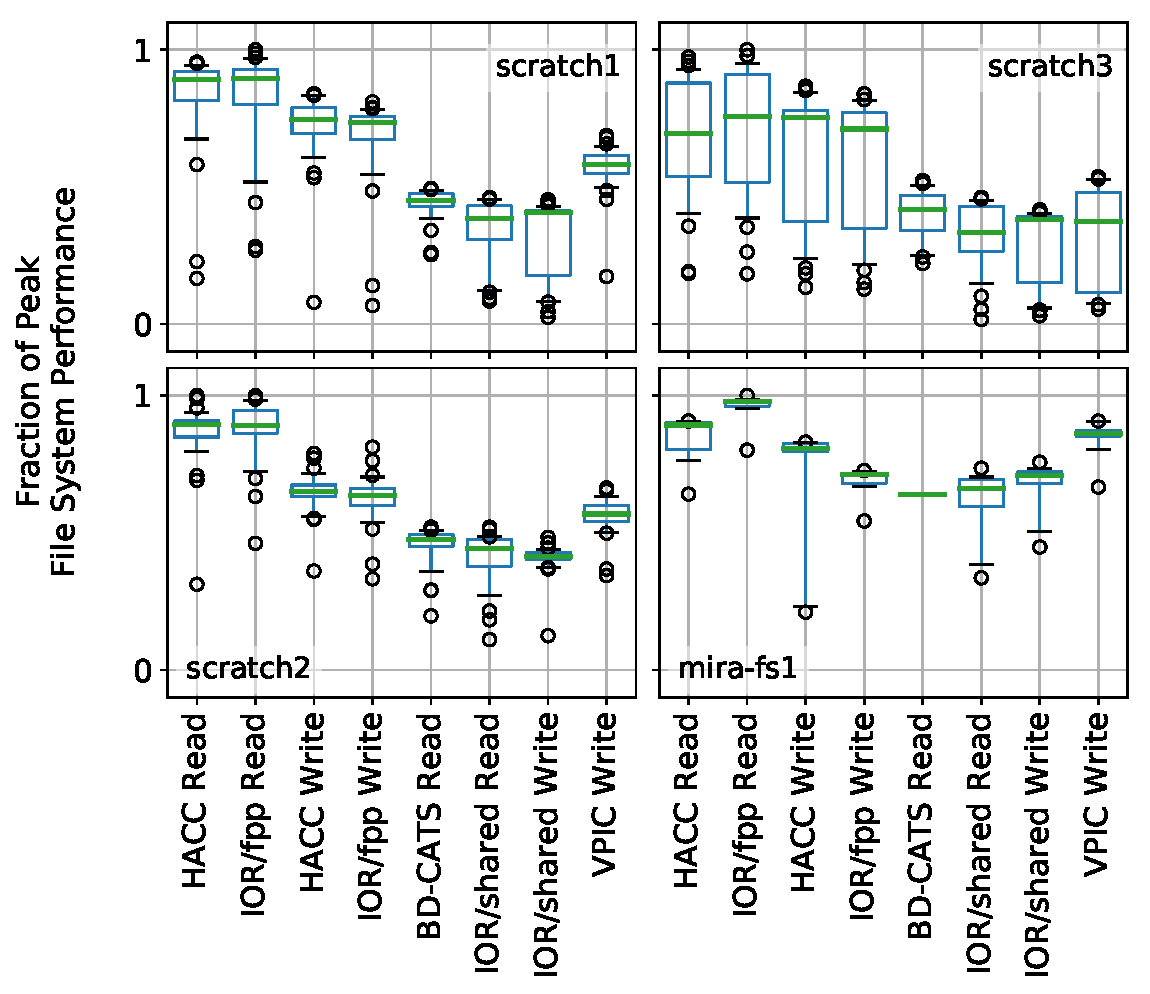
\includegraphics[width=1.0\columnwidth]{figs/perf-boxplots-per-fs.pdf}
    \caption{TOKIO-ABC I/O performance for Edison (\texttt{scratch1},
    \texttt{scratch2}, \texttt{scratch3}) and Mira (\texttt{mira-fs1}) normalized to
    the mean of all tests performed on each file system.  Each box reflects the
    distribution of all four application workloads and both read and write
    performance. Whiskers represent the 5th and 95th percentiles.}
    \label{fig:perf-summary-boxplots-fs}
\end{figure}

Such variation in peak file system performance caused by suboptimal I/O access patterns is well documented\cite{Lofstead2010,Uselton2010,Xie2012}.
To focus solely on the variation caused by factors \emph{extrinsic} to each application, we then define the \emph{fraction of peak performance} as the performance of a job divided by the maximum performance observed for all jobs \emph{of the same I/O motif} as listed in Table \ref{tab:bench-config} and whether the job did reads or writes.
For example, the fraction peak performance for a HACC write test is only normalized to the maximum performance of all other HACC write tests.
References to fraction peak performance are hereafter defined this way.

This fraction of peak performance distribution, shown in Figure~\ref{fig:perf-summary-boxplots-motif}, reveals that the degree of performance variation \emph{within} each application also varies with each file system.
For example, the HACC write workload is susceptible to a long tail of performance degradation on mira-fs1 despite
that file system's overall lower variation shown in Figure~\ref{fig:perf-summary-boxplots-fs}.
Similarly, all Edison file systems show a long tail of performance loss for the IOR/shared file read workload.
Edison's scratch3 also demonstrates very broad performance variation for the VPIC write workload, contrasting with the relatively narrow performance variation of this application on all other file systems.

\begin{figure}[t]
    \centering
    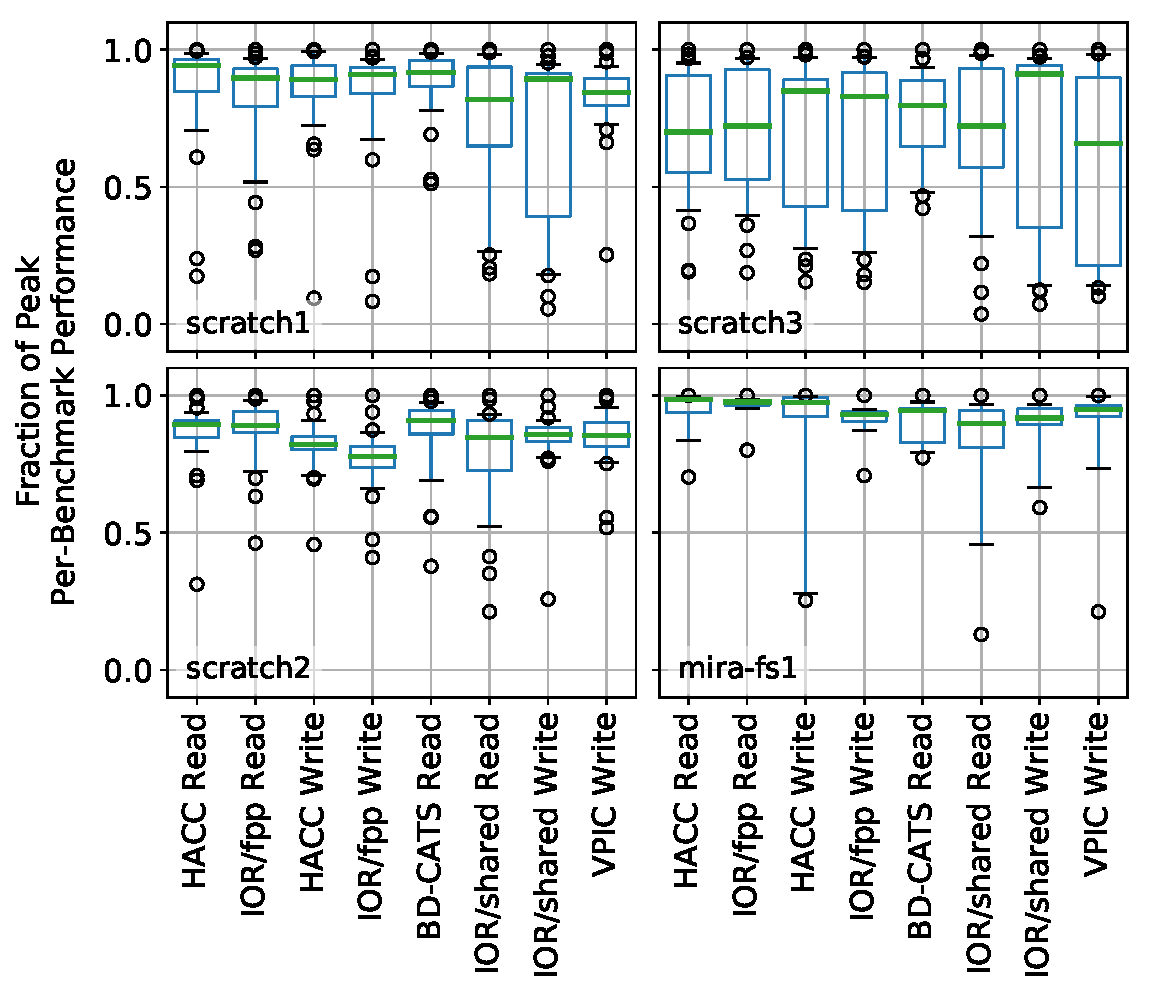
\includegraphics[width=1.0\columnwidth]{figs/perf-boxplots.pdf}
    \caption{TOKIO-ABC I/O performance for all file systems tested grouped by test
    applications and read/write mode.  Whiskers represent the 5th and 95th
    percentiles.}
    \label{fig:perf-summary-boxplots-motif}
\end{figure}

\textbf{Thus, Figure \ref{fig:perf-summary-boxplots-motif} demonstrates that the
performance variability results from factors intrinsic to the application (e.g., I/O motif) \emph{and} factors intrinsic to the file system}, and
different I/O motifs result in different levels of performance \emph{and} variability.
Furthermore, these behaviors are not a function of the parallel file system software architecture either; all Edison file systems are Lustre-based, and yet there is a marked difference in variability between scratch1/scratch and scratch3 shown in Figure~\ref{fig:perf-summary-boxplots-motif}.
Thus, these differences in performance variation must be a result of their different hardware configurations (discussed in Section \ref{sec:platforms}), their specific user workloads, or a combination of both.

%%%%%%%%%%%%%%%%%%%%%%%%%%%%%%%%%%%%%%%%%%%%%%%%%%%%%%%%%%%%%%%%%%%%%%%%%%%%%%%%
\subsection{Combining Application and Server-side Telemetry} \label{sec:results/combining}
%%%%%%%%%%%%%%%%%%%%%%%%%%%%%%%%%%%%%%%%%%%%%%%%%%%%%%%%%%%%%%%%%%%%%%%%%%%%%%%%

To obtain a better understanding of how performance variation is caused by factors extrinsic to the application, we then combine what we know from application-level analysis provided by Darshan with file system-level analysis provided by LMT (on Edison) and ggiostat (on Mira).  An intuitive source of performance loss would be from other jobs that are also consuming file system bandwidth, so to explore the effects of competing I/O traffic, we define the \emph{coverage factor} ($\mathit{CF}$) of a job $j$:

\begin{equation} \label{eq:cf}
    \mathit{CF}(j) = \frac{N_{\textup{bytes}}^{\textup{Darshan}}(j)}
    {\sum_{t,s}^{\textup{time,servers}}
    \left [ N_{\textup{bytes}}^{\textup{LMT,ggiostat}}(t,s) \right ] }
\end{equation}
%
where $N_{\textup{bytes}}^{\textup{Darshan}}$ is the number of bytes read and written by job $j$ according to its Darshan log, and $N_{\textup{bytes}}^{\textup{LMT,ggiostat}}$ is the number of bytes read and written to a parallel file system server $s$ during a 5-second time interval $t$.
The time interval over which the job ran ($\mathit{time}$) and the servers to which the job wrote ($\mathit{servers}$) are both taken from the job's Darshan log~\cite{snyder2016modular}.

The coverage factor is a direct reflection of how much I/O traffic a job
competed against in the underlying file systems.  $CF = 1.0$ when
all of the server-side I/O was caused by job $j$, while $CF = 0.5$ indicates that only half of the server-side I/O was attributable to job $j$ while the other half came from other sources.
In practice, it is possible to observe $CF > 1.0$ 
if (1) server-side monitoring (e.g., LMT or ggiostat)
did not capture data from all servers during a polling interval, or (2) clock skew exists between the compute nodes and the file system servers, causing the Darshan log and LMT/ggiostat to have an inconsistent understanding of when I/O happened.
To eliminate the most erroneous data, we discard all test results where $CF > 1.2$ in the subsequent analysis.
\todo{We should probably mention what \% of data this covers. It will be a likely question.}

The distribution of coverage factors across all experiments run are shown in
Figure~\ref{fig:cdfs}a which reveals that the majority of tests
($> 85\%$ on Edison and $> 75\%$ on Mira) have high coverage factor
($CF > 0.90$).  This is consistent with the observation that I/O occurs in
bursts~\cite{Carns2011,Liu2016}, and the probability of two bursts coinciding
and causing contention for bandwidth (thereby reducing $CF$) is relatively low.
In particular, Mira's CF distribution is so narrow that over 50\% of tests effectively ran completely uncontended for bandwidth; $\textit{CF} >= 0.99$ corresponds to the 43rd percentile on that system.

Despite this low incidence of overlapping bursts, though, the cumulative
distribution function (CDF) of performance relative to the peak observed
bandwidth for each application (Figure~\ref{fig:cdfs}b) is far more broadly distributed.
Between 19\%-23\% (scratch1/scratch2) and 47\% (scratch3) of jobs on Edison got less than half of the peak observed performance, clearly indicating that the coverage factor (and therefore server-side
I/O bandwidth) is not the only contributor to sub-optimal performance.  
This finding is consistent with
the work of Uselton and Wright\cite{Uselton2013} who demonstrated that Lustre
file system performance is constrained by both the weighted sum of both bandwidth
\emph{and} I/O operation (IOP) rate.  

\begin{figure}[t]
    \centering
    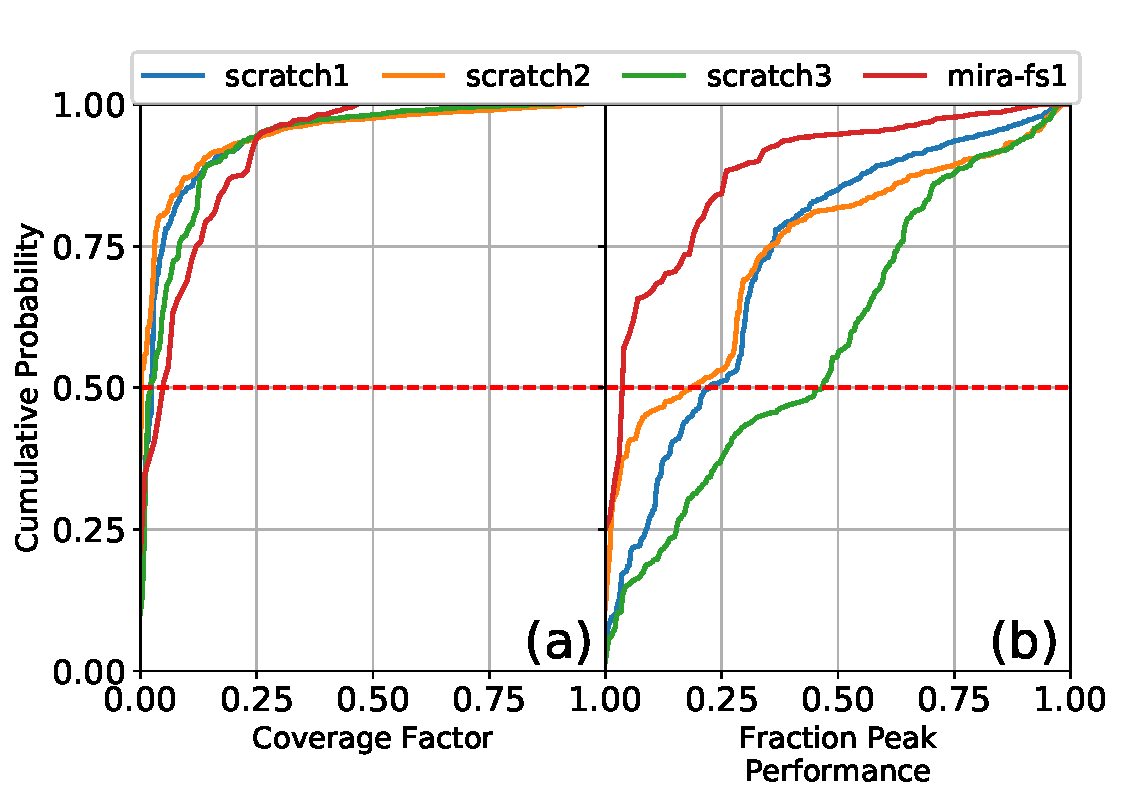
\includegraphics[width=\columnwidth]{figs/cdf-both.pdf}
    \caption{Cumulative distribution function of the coverage factor (a) and the
    performance relative to the maximum throughput observed across each file system
    (b).  The line demarcating 50\% probability corresponds to coverage factors of
    \todo{UPDATE}0.028, 0.004, 0.015, and 0.050 and peak performance fractions of 0.227, 0.185,
    0.467, and 0.040 on Edison scratch1-scratch3 and Mira, respectively.}
    \label{fig:cdfs}
\end{figure}

\begin{figure}[t]
    \centering
    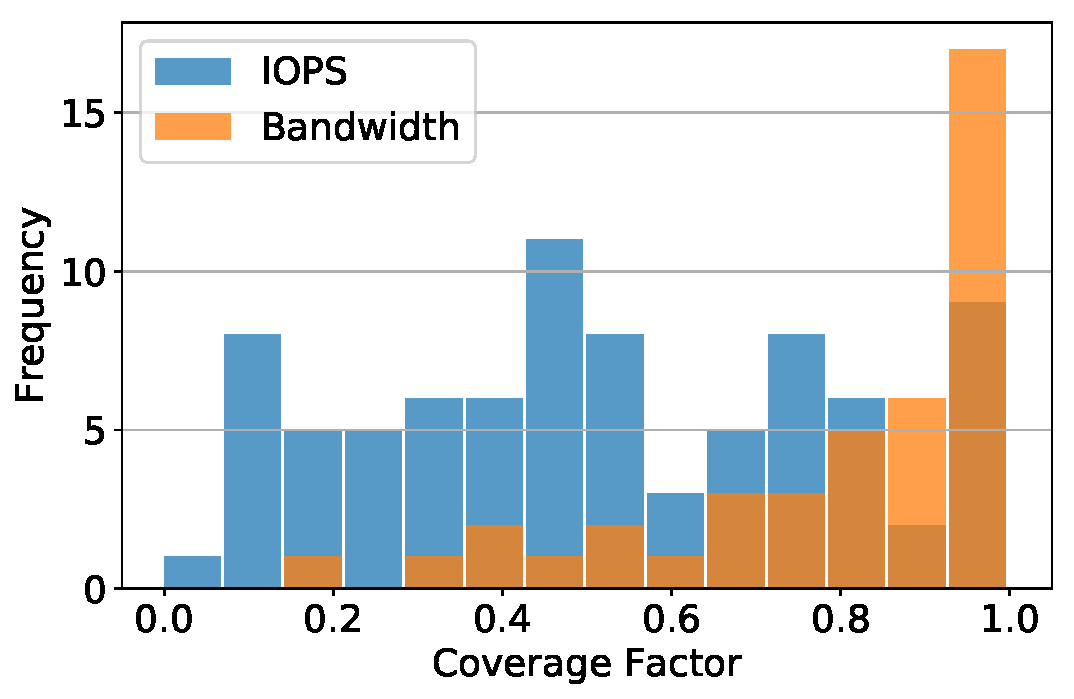
\includegraphics[width=\columnwidth]{figs/hist-cf-bw-and-ops.pdf}
    \caption{Distribution  of the coverage factor for both bandwidth ($\textit{CF}_{\textup{bandwidth}}$) and read/write operations ($\textit{CF}_{\textup{iops}}$) for Mira.
    }
    \label{fig:hist-cf-mira}
\end{figure}

To understand the relationship between IOP contention and performance degradation, we can also calculate the coverage factor of IOPS in addition to the coverage factor of bandwidth described in Equation \ref{eq:cf}.
If the relationship between performance and bandwidth is proportionately affected by IOPS-based contention, we would expect the coverage factor of IOPS to follow a similar distribution.
However, as shown in Figure \ref{fig:hist-cf-mira}, $\textit{CF}_{\textup{iops}}$ for Mira jobs are broadly distributed, whereas $\textit{CF}_{\textup{bandwidth}}$ shows a clear bias towards high values.
From this, we can conclude that many tests on Mira achieved high performance despite other I/O loads concurrently generating commensurate IOP loads.
Thus, high background IOPS can be a cause for performance loss, but their presence do not necessarily preclude achieving high performance.

% We should point out that the coverage factor for IOPS is more ambiguous than
% the coverage factor for bandwidth because file system clients are able to
% coalesce many small transactions into a single large transaction.  Although
% we don't see this happen on IOR, HACC, or VPIC, the BDCATS-IO benchmark
% issues a TON of small (512-byte) transactions (per Darshan) that do not
% appear on the server side.

%%%%%%%%%%%%%%%%%%%%%%%%%%%%%%%%%%%%%%%%%%%%%%%%%%%%%%%%%%%%%%%%%%%%%%%%%%%%%%%%
\subsection{Correlating Different Data Sources} \label{sec:results/correlating}
%%%%%%%%%%%%%%%%%%%%%%%%%%%%%%%%%%%%%%%%%%%%%%%%%%%%%%%%%%%%%%%%%%%%%%%%%%%%%%%%

\todo{need to explicitly acknowledge the limitations, suitability, and extent of our confidence in the statistical methods employed here.}

Our choice to define our correlation parameter according to application performance and server-side bandwidth and IOPs was motivated by a broad body of literature and an intuitive assumption that competition for bandwidth and IOPs affect performance the most dramatically.
However, the TOKIO framework is generalized to draw data from any resource that can be indexed on a per-job or time series basis.
As such, we can attempt to correlate a wide variety of measurements to job I/O performance to determine which measurements are likely culprits when looking for sources of poor I/O performance.

To this end, we calculated the Pearson correlation coefficient between each job's fraction of peak performance (as defined in Section \ref{sec:results/overview} ) with a wide range of metrics collected on Edison and Mira, and the most interesting results are summarized in Figure \ref{fig:correlation-table}.
Although an exhaustive examination of all correlations is beyond the scope of this work, several key points can be gleaned by what these data do \emph{and do not} show.

\begin{figure}[t]
    \centering
    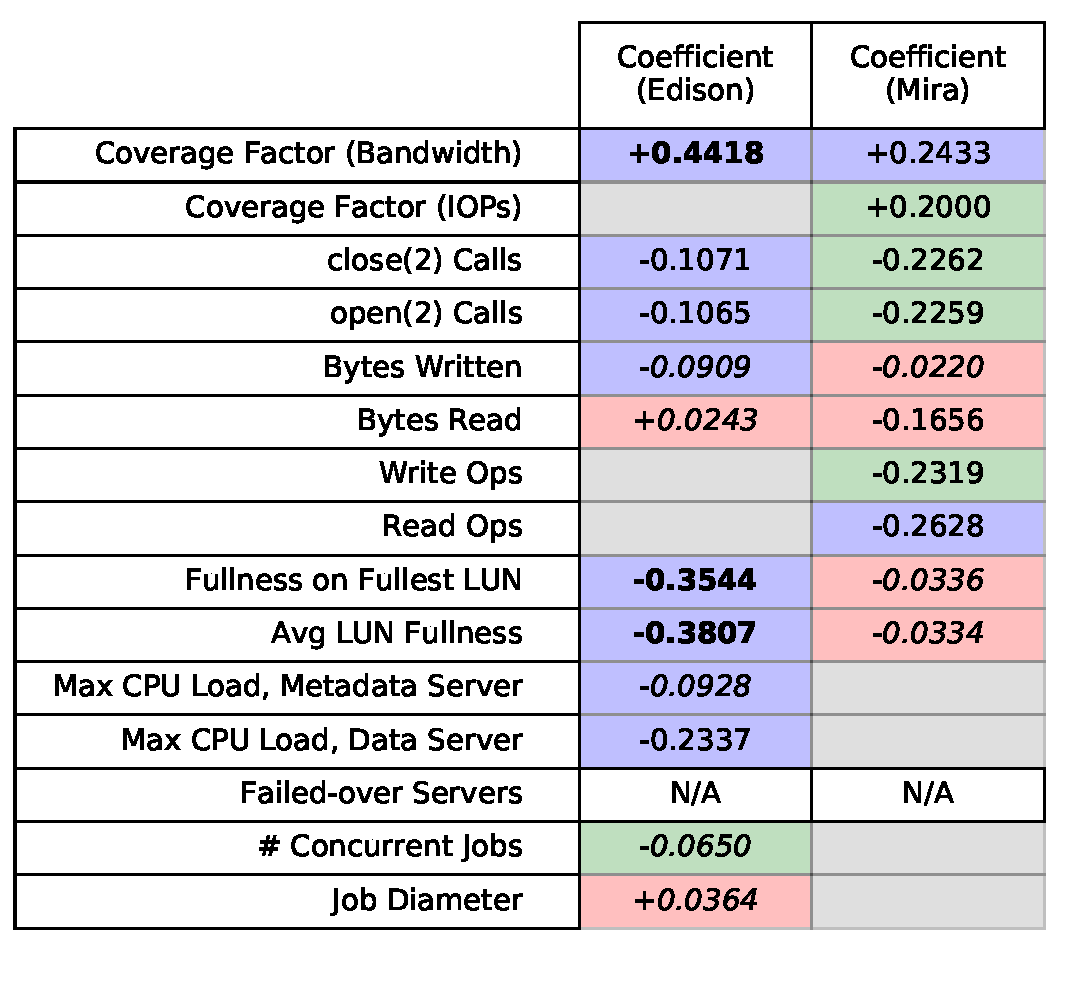
\includegraphics[width=\columnwidth]{figs/correlation_table.pdf}
    \caption{Correlation coefficients between fraction of peak performance measured for each I/O motif and a variety of server-side measurements and metrics.  Box color indicates confidence; correlations with p-values $< 0.01$ are blue; p-values $< 0.05$ are green, and p-values $>= 0.05$ are red (and signify lack of correlation).  Similarly, bolded values signify moderate correlation ($|r| > 0.30$), and italicized values signify weak correlation ($|r| < 0.10$).  Although the "\% Servers Failed Over" measurement were tracked on both Mira and Edison, no changes in the
    failover states of servers were ever observed over the course of this study.
    }
    \label{fig:correlation-table}
\end{figure}

\begin{itemize}

\item As assumed in the previous sections, the coverage factors correlate most strongly with performance on all file systems, indicating that contending for file system I/O is a moderate contributor to performance loss.
Mira's file system also demonstrated moderate sensitivity to contention for IOPs; unfortunately, Lustre IOPs were not collected for this study, so no comparison can be made to Edison.

\item Mira's performance correlates negatively with higher rates of \texttt{open(2)}/\texttt{close(2)} calls than Lustre.
Given that Mira's file system encodes metadata in the same physical servers as data blocks, this relationship is reasonable.
By comparison, Edison's file systems each have their own discrete metadata servers are specifically designed to decoupled bulk data transfer performance from metadata operations.

\item The fullness of each storage device (LUN on Mira and OST on Edison) has markedly different behavior between Edison and Mira.
While Mira's performance is uncorrelated with device capacity, Edison performance degrades as free space on OSTs is depleted.
This is a documented behavior of Lustre file systems.

\item Perhaps contrary to historic intuition, I/O performance shows no meaningful correlation with the number of other jobs running concurrently.
The lack of correlation with concurrent job count is consistent with our finding that I/O remains highly bursty; a large number of small jobs are highly unlikely to burst simultaneously, and each small job is not individually capable of impacting our tests' coverage factors.

\item Similarly, the job diameter (a measurement of how spread out a job is across the compute fabric) has no discernible correlation with I/O performance on Edison.
Given the fact that the low-diameter dragonfly topology of Edison is designed to reduce the performance impact of job topology, this is consistent with expectation.

\end{itemize}

In addition to the measurements and metrics presented in Figure \ref{fig:correlation-table}, the TOKIO framework collected a larger number of system-specific measurements that did not correlate significantly to performance.
However it is important to underscore the fact that this demonstration was not intended to be exhaustive, and the correlations and p-values for the Edison system are likely diminished by the fact that all three Edison file systems, each with unique users, workloads, and governance policies, were combined for this analysis.

%%%%%%%%%%%%%%%%%%%%%%%%%%%%%%%%%%%%%%%%%%%%%%%%%%%%%%%%%%%%%%%%%%%%%%%%%%%%%%%%
\subsection{Unified Measurements and Metrics Interface} \label{sec:results/umami}
%%%%%%%%%%%%%%%%%%%%%%%%%%%%%%%%%%%%%%%%%%%%%%%%%%%%%%%%%%%%%%%%%%%%%%%%%%%%%%%%

By establishing an understanding of the baseline distribution of performance for each I/O motif and file system in Sections \ref{sec:results/overview} and \ref{sec:results/combining} and identifying how different measurements and metrics correlate with performance in \ref{sec:results/correlating}, we now have a foundation from which we can describe

\begin{enumerate}
\item where on the spectrum of normalcy a specific job's I/O behavior fell relative to other jobs with a similar I/O motif, and
\item which measurements and metrics are the best places to start investigating abnormal conditions based on how they have historically correlated with performance
\end{enumerate}

\begin{figure}[t]
    \centering
    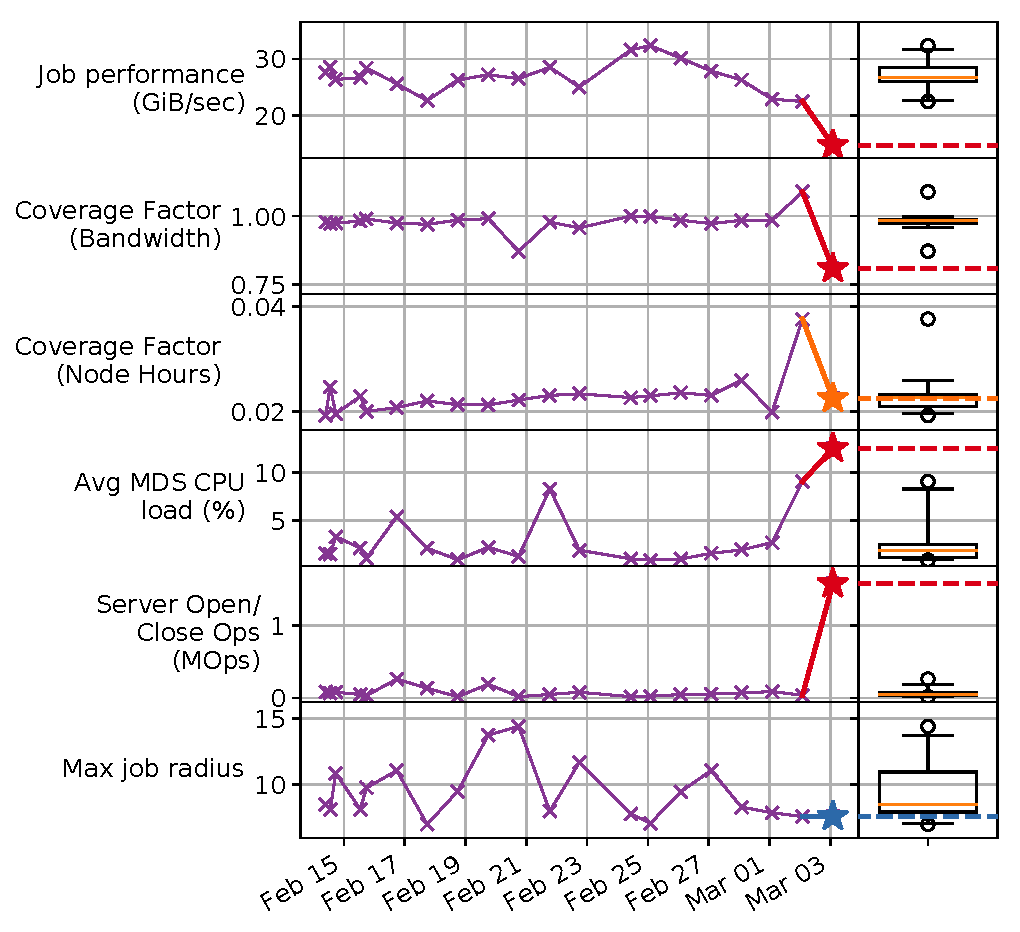
\includegraphics[width=1.0\columnwidth]{figs/umami-scratch2-hacc-write.pdf}
    \caption{TOKIO-UMAMI demonstrating the \emph{file system climate} of HACC write workloads
    on the Edison scratch2 file system compared to a most recent run, which showed
    highly unusual \emph{file system weather}.}
    \label{fig:umami-scratch2-hacc-write}
\end{figure}

To concisely visualize all of this information, we present the TOKIO Unified Measurements and Metrics Interface (UMAMI), shown in Figure \ref{fig:umami-scratch2-hacc-write}, with the goal of enabling end-users to quickly see how their application's performance compares to similar I/O workloads in the past.
TOKIO-UMAMI presents historic measurements from the components monitored by TOKIO, composing what we refer to as the \emph{I/O subsystem climate}, and summarizes each metric's distribution in a box plot to the right of each metric's time series plot.
These time series plots terminate with the measurements taken for the job in question, describing the \emph{I/O subsystem weather} at the time that job ran.
By overlaying this weather on the climate box plots in the form of dashed lines, TOKIO-UMAMI provides a quick visualization of how each metric's weather compared to the statistical distribution of past weather conditions.
This conceptualization of a file system's weather with its overall climate, a user can differentiate between a long-term performance problem (as would occur if the application I/O is not optimized for the underlying file system) and a statistically rare event analogous to an extreme weather event.

The specific UMAMI example shown in Figure \ref{fig:umami-scratch2-hacc-write} represents a HACC write test which took place on March 3.
This particular job showed abnormally low performance as evidenced by the "Job performance (GiB/sec)" measurement and its value relative to the previous six instances of this type of job.
This abnormally poor job performance was accompanied by an unusually low coverage factor and high metadata load, and these unfavorable conditions (which fell into the bottom-most quartile of past measurements) are highlighted as red dashed lines in the box plots.
The metrics corresponding to blue dashed lines fell into the uppermost quartile for this problematic job, but as discussed in Section \ref{sec:results/correlating}, have no history of correlation with performance.
Thus, we can quickly attribute the poor performance of this HACC job to an I/O extrinsic to this HACC job which was competing for both bandwidth on the data servers and metadata resources on the metadata server.

Similarly, Figure \ref{fig:umami-mira-fs1-vpic-write} represents a VPIC write workload that showed poor performance on Mira.  However, its coverage factor is within normal parameters (the orange lines in each metric's box plot signifies a value in the second quartile) indicating a general lack of bandwidth contention.  Although the IOPS coverage factor is also abnormally low, previous conditions have been worse despite a lack of dramatic performance loss (e.g., on March 7).  The only metric that shows a unique, undesirable value is the number of \emph{readdir(3)} operations handled by the file system.  This is indicative of an expansive file system traversal and was demonstrated to correlate moderately negatively with performance in Figure \ref{fig:correlation-table}.

\begin{figure}[t]
    \centering
    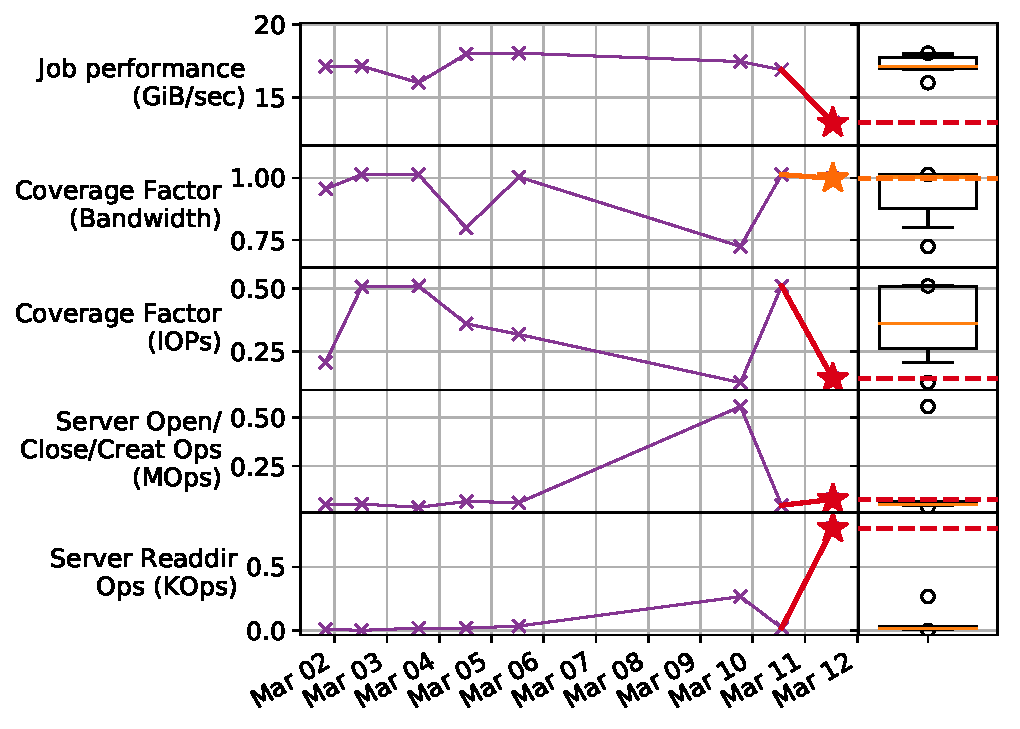
\includegraphics[width=1.0\columnwidth]{figs/umami-mira-fs1-vpic-write.pdf}
    \caption{TOKIO-UMAMI demonstrating the \emph{file system climate} of VPIC-IO write workloads
    on Mira compared to a most recent run, which showed
    highly unusual \emph{file system weather}.}
    \label{fig:umami-mira-fs1-vpic-write}
\end{figure}

%%%%%%%%%%%%%%%%%%%%%%%%%%%%%%%%%%%%%%%%%%%%%%%%%%%%%%%%%%%%%%%%%%%%%%%%%%%%%%%%
\subsection{Discussion} \label{sec:results/discussion}
%%%%%%%%%%%%%%%%%%%%%%%%%%%%%%%%%%%%%%%%%%%%%%%%%%%%%%%%%%%%%%%%%%%%%%%%%%%%%%%%

This section will discuss \emph{why} we saw the behavior that we did by
aligning and correlating data sources, then make broader conclusions about the
differences between Mira and Edison results.

Overall, instances of abnormally poor I/O performance on Mira were most often attributable to equally abnormal coverage factors (indicating bandwidth contention) or high metadata rates (opens/closes and readdirs).  Of all \todo{UPDATE}92 tests run on this file system, only one case of performance falling in the first quartile was not accompanied by one of these server-side contention conditions.

The most common sources of performance loss on Edison were more difficult to neatly categorize because server-side IOPS were not measured explicitly.  In those cases where performance was poor despite a high coverage factor, many secondary indicators of high IOPS load (such as high data server CPU load and high metadata rates) were observed.  For example, Figure \ref{fig:umami-deepdive} shows a "deep-dive" view of a particular VPIC run that showed a 3x performance loss.  By showing a server-side, time-resolved trace of write bandwidth on a per-OST basis, we see that there are no straggling writers as is often implicated in collective I/O.  Rather, the bubbles are likely due to a server-side blocking situation, such as journal flushing, which would arise from a high rate of small I/O transactions from another source filling the journal on one or more Lustre OSSes.
\todo{show the good deepdive heatmap too}

\begin{figure}[t]
    \centering
    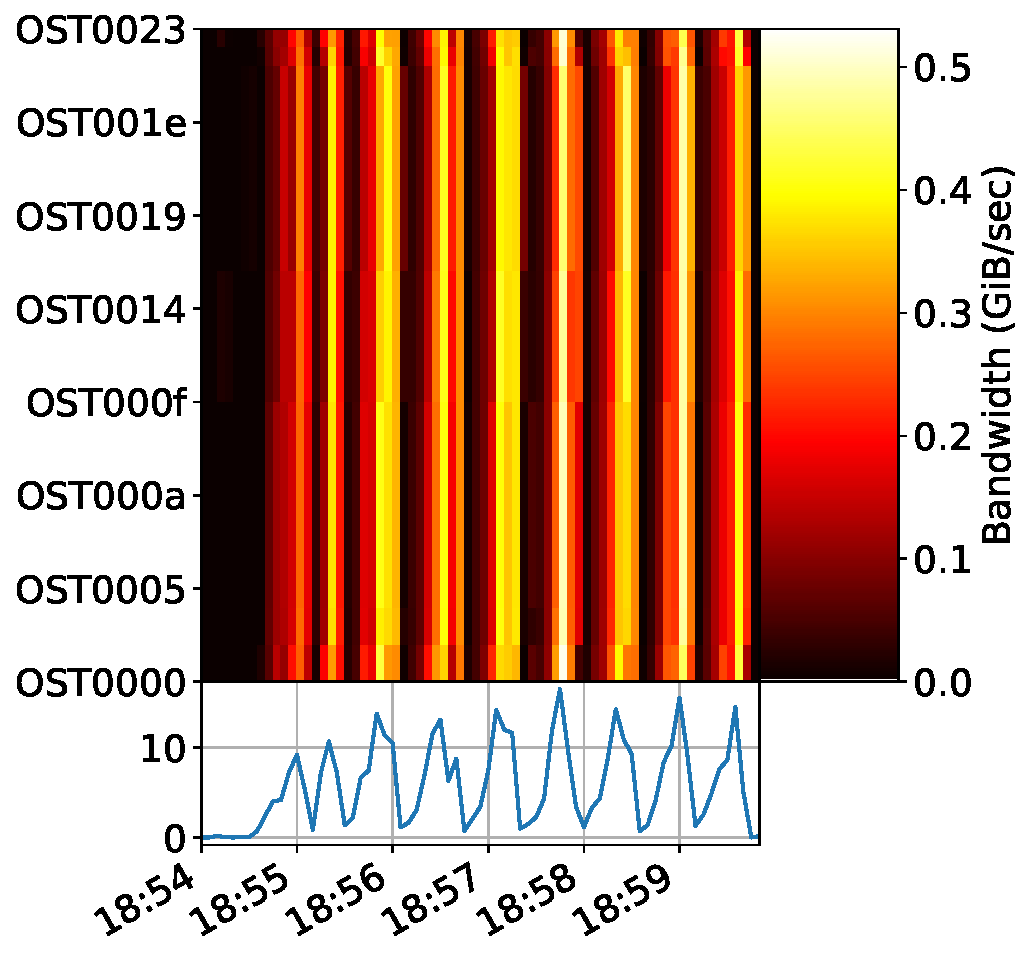
\includegraphics[width=1.0\columnwidth]{figs/deepdive-scratch3-vpic-write_feb24.pdf}
    \caption{TOKIO-UMAMI time resolved view of a poorly performing VPIC job.  Each row in the heat map corresponds to an OST, and the line graph represents the sum over all OSTs at each time step.  Each I/O burst corresponds to writing out a single VPIC variable (see \ref{sec:methods/tests}) and, under normal conditions, does not demonstrate the discrete bubble of low bandwidth after each write operation.}
    \label{fig:umami-deepdive}
\end{figure}

The TOKIO framework was also able to identify longer-term performance issues which progressively degraded write performance. Figure \ref{fig:umami-scratch3-hacc-write-long-term} shows the UMAMI view such an event on Edison's scratch3 file system where coverage factors were not highly abnormal despite an ongoing 2x slowdown over the normal 50 GIB/sec.  The magnitude of performance loss followed the highest CPU load observed across all of the Lustre OSSes almost exactly, and this period coincided also with the scratch3 file system reaching critical levels of fullness.  Although such correlations cannot define causative relationships, these conditions indicated a relationship between critically full storage devices and CPU load (e.g., an increasing cost of scavenging empty blocks) that impacts application performance, consistent with our understanding of how Lustre performance degrades with increasing OST fullness.

\begin{figure}[t]
    \centering
    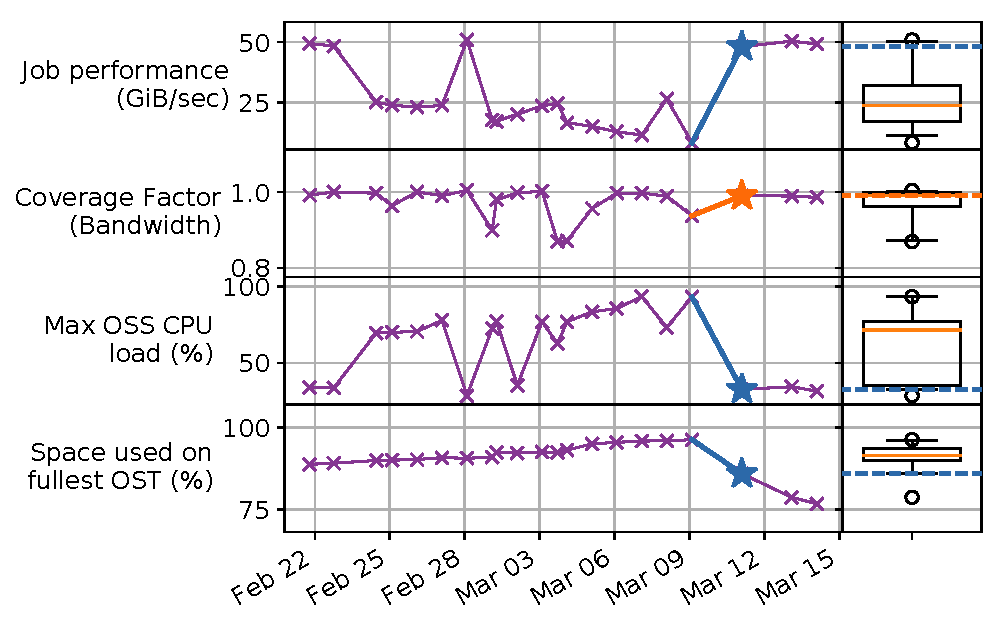
\includegraphics[width=1.0\columnwidth]{figs/umami-scratch3-hacc-write-long-term.pdf}
    \caption{TOKIO-UMAMI of HACC write performance on Edison's scratch3 file system showing a longer-term period of performance degradation that was associated with unusually high OSS CPU load.}
    \label{fig:umami-scratch3-hacc-write-long-term}
\end{figure}

Qualitatively, the highly variable I/O workload and "I/O weather" conditions across the Edison file systems obfuscate a straightforward analysis of all of the sources of performance variation on its file systems.  Over the course of this study, we found that the TOKIO framework often exposed variation resulting from the confluence of several factors that only correlate weakly with performance when examined independently.  Thus, TOKIO requires some amount of expert knowledge to confidently determine the root cause of I/O problems on file systems that are subject to large amounts of incoherent or otherwise noisy I/O.  That said, presenting the historic correlations between performance and each variable through UMAMI does dramatically reduce the exploration space in this effort.

Capturing an historic record of a file system's climate for a particular workload is not always straightforward, and at present, users will have to self-identify jobs and Darshan logs that should be used to build this historic record.  Alternatively, UMAMI can be seeded with data from baseline performance tests, as was done in this study, provided that the user's I/O motif is sufficiently similar to one of the baseline tests' motifs.  This can be automated to a large degree though; the simplest approach is to scan Darshan logs for similar I/O transaction size distributions as seeds.  Recently, Liu et al
have also demonstrated combining resource manager logs and
server-side I/O logs to identify a series of I/O bursts with specific jobs using a density-based clustering method~\cite{Liu2016}.  We believe that adapting this clustering-based classification approach with TOKIO-UMAMI should be a straightforward approach to building an I/O climate record for any arbitrary job.

Finally, although we applied TOKIO and UMAMI to build I/O climate histories specific to applications based on Darshan logs, it is equally possible to group historic data around similar periods of server-side traffic.  For example, TOKIO can be used to identify collections of applications that, when run together,
result in an uncommonly adversarial I/O load or, conversely, surprisingly
good performance.  From this, it is easy to envision an opportunity to inform job scheduling
to avoid I/O contention between two frequently conflicting applications.

% \begin{itemize}
% \item Sometimes metadata operations are slow (e.g., file-per-process I/O)
%     \begin{itemize}
%     \item Show Darshan logs showing high metadata time
%     \item Show LMT MDT logs showing high background metadata or CPU rate
%     \item Show GPFS NSD metadata loads?  Can we do this?
%     \end{itemize}
% \item Sometimes hardware goes bad
%     \begin{itemize}
%     \item Show Darshan logs showing bad performance at the POSIX layer (i.e., not the
%     application's fault)
%     \item Show Lustre OSTs that stall out
%     \item Show slow Lustre OSTs due to failover/oversubscription (a la Darshan 3 paper)
%     \item Show poorly performing GPFS NSDs
%     \end{itemize}
% \item Sometimes there is interference from other applications
%     \begin{itemize}
%     \item Show Darshan logs showing bad performance at the POSIX layer (i.e., not the
%     application's fault)
%     \item Show jobs with and without background LMT load
%     \item Show jobs with and without background mmpmon load
%     \end{itemize}
% \item Sometimes tuning strategies differ across platforms
%     \begin{itemize}
%     \item contrast which benchmark performs best on each platform
%     \item dig into why
%   \item See example of how we might show this in Figure~\ref{fig:example-bar-var}
%     \end{itemize}
% \end{itemize}
